\section{Test set-up}
\label{sec:setup}
\begin{figure}[h!] 
\center  
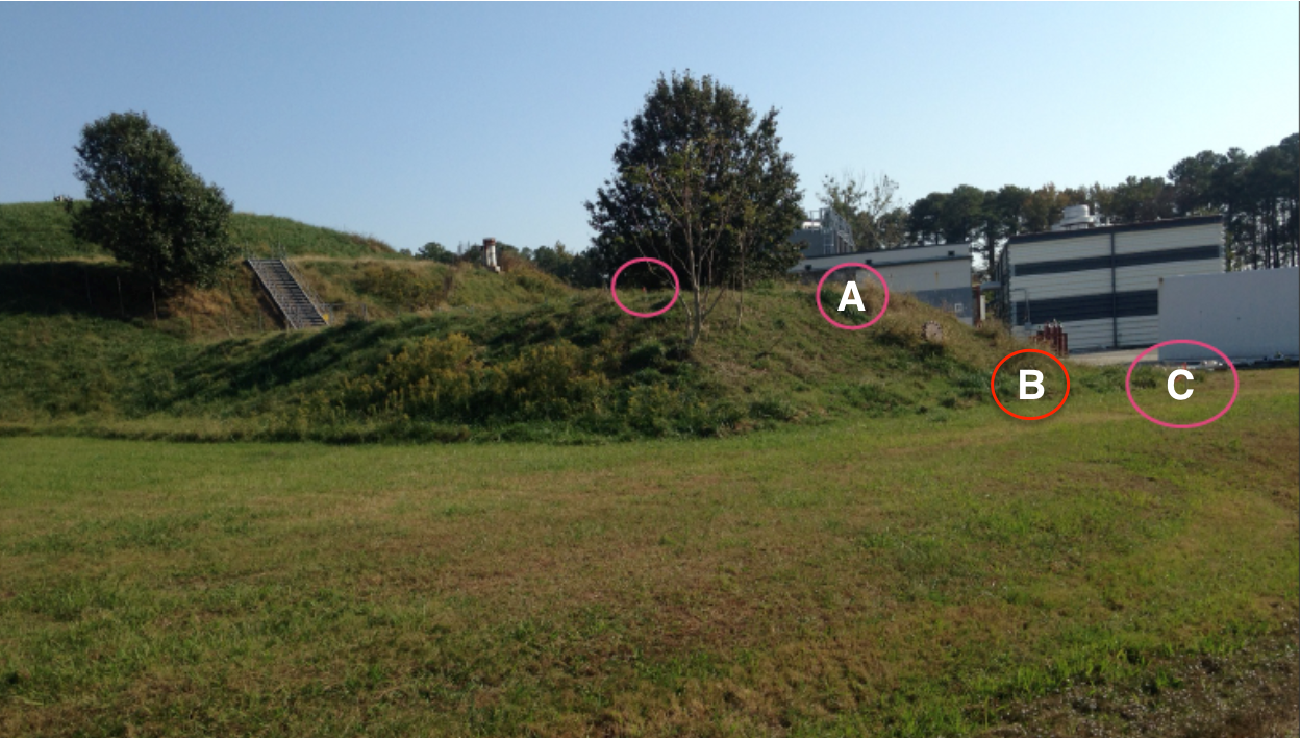
\includegraphics[width=11.5cm]{figs/ds-area.pdf}   
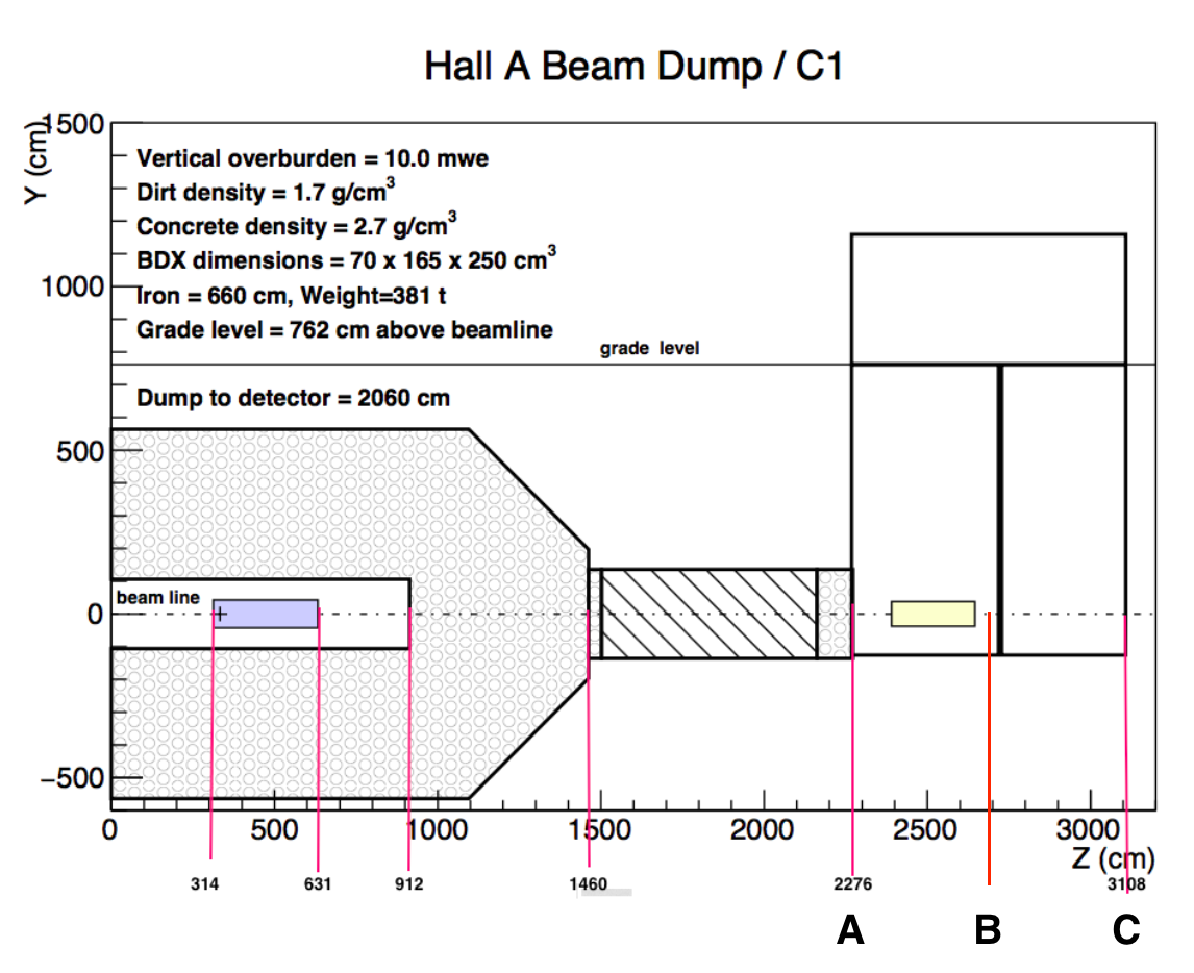
\includegraphics[width=11.5cm]{figs/test-plan.pdf}  
\caption{The area downstream of the Hall-A beam-dump and the studied test locations.}
\label{fig:ds-area}
\end{figure} 

\subsection{Detector location}
The area downstream of Hall-A beam-dump is shown in Fig.~\ref{fig:ds-area}  indicating test measurement locations relative to the 
new  underground facility proposed in PR-16-001~\cite{bdx-proposal}. The three positions, indicated with markers {\bf A, B}  and {\bf C},  correspond to the hall entrance (22.4 m downstream of the beam-dump entrance), a point in the middle  (25.2 m) and the exit (28 m), respectively. The experimental set-up we are proposing requires digging a well and inserting a pipe in one (or more) of these locations. The BDX-Hodo detector will be lowered in the pipe and the muon flux sampled at different heights wrt. nominal beam height. The muon flux profiles in Y (vertical direction), measured in  different locations in Z (distance from the dump), will allow us to compare the absolute and relative MC predictions. 

\subsection{The BDX-Hodo detector \label{sec:BDX-hodo}}
The detector used to measure the beam-on-related muon radiation and the background in the proximity of the new BDX underground facility will  make use of a BDX ECal CsI(Tl) crystal sandwiched between a set of segmented plastic scintillators.
A CAD representation as well as  a vertical and horizontal  cut with dimensions are shown in Fig.~\ref{fig:det-cad}.
\begin{figure}[h!] 
\center
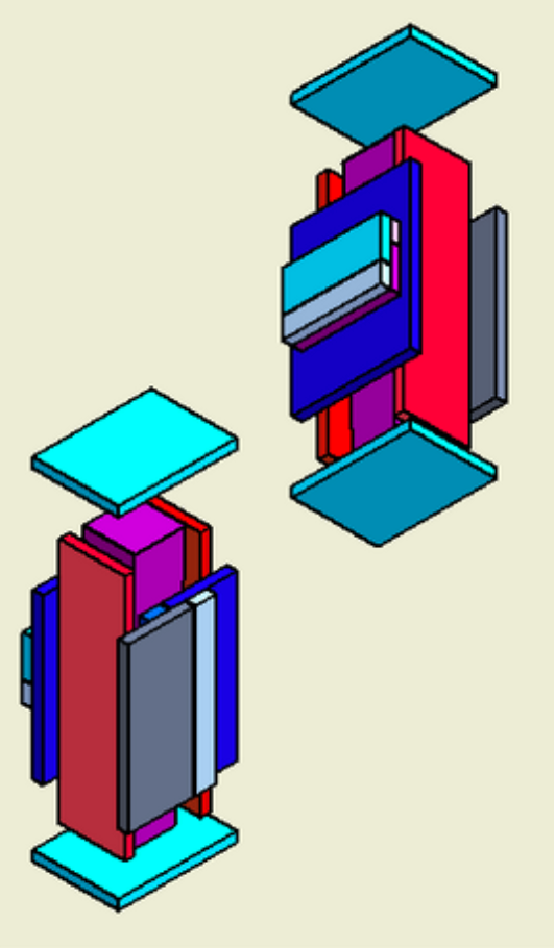
\includegraphics[width=3.3cm]{figs/det-3d1.pdf}  
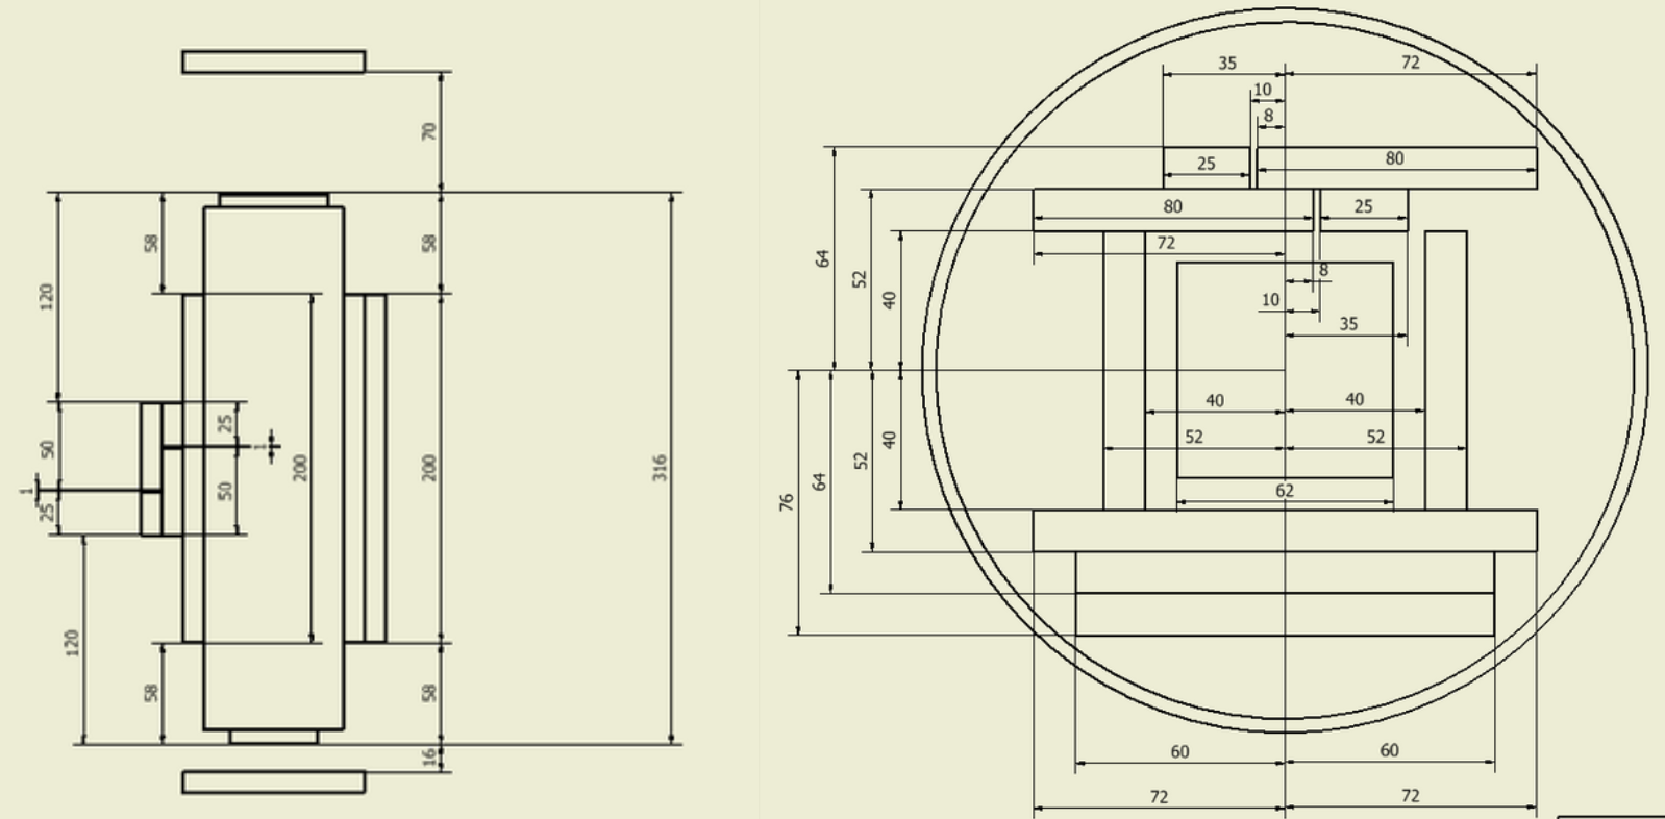
\includegraphics[width=11.5cm]{figs/det-3d2.pdf}   
\caption{The CAD representation of the BDX-Hodo detector and some drawings with geometry and sizes.}
\label{fig:det-cad}
\end{figure}
The front of the crystal will be equipped with two  layers of plastic scintillators, each composed by  a large and a small 1 cm-thick scintillators strips. The overlap of the four paddles (each 20 cm long in Y)  results in three independent  2.5 cm channels along the X (horizontal) direction.
The same concept was applied to the  back side of the crystal but with paddles tilted by 90 degrees to define three 2.5 cm independent channels along the Y (vertical) direction. The requirement of a hit in both front and back paddles defines a 3x3 matrix of 2.5x2.5 cm$^2$ pixels providing a cm-like muon XY position resolution. 
The addition of a larger paddle (20 x 14.4 cm$^2$) on the back provides an enhanced sensitivity   in the unlikely  case rates will be much lower than what estimated by MC simulations.
Four more  paddles covering  the left/right sides and the top/bottom of the crystal will be used to veto cosmic rays and other radiation not associated to the beam direction.
The crystals will be coupled, on the large side,  to a 6x6 mm$^2$ Hamamatsu S13360-6025 SiPM as described in Sec. 3.2.1 of  PR-16-001~\cite{bdx-proposal}. The scintillator paddles will be  made with extruded plastic, each  read out via a WLS fiber coupled to a 3x3 mm$^2$ Hamamatsu S12572-100 SiPM sharing the same technology used in the BDX Inner Veto detector (described in details in Sec. 3.2.2 of  PR-16-001).
The detector will be contained  in a 20-cm diameter stainless-steel cylindrical vessel, covered on top and on the bottom by steel lids. The whole assembly will  be water-tight to prevent any water from leaking inside the vessel. A stainless-steel  extension on the top cover will be used  to run  cables (signal and power)  from the detector to the ground-level. The extension, made by a 1-inch stainless steel pipe,  rigidly attached to the whole assembly, will be also used  to remotely control the cylinder orientation  providing correct  the alignment of the BDX-Hodo wrt. the beam axes. \\
To record the 13 (scintillators) + 1 (crystal) channels a  single 16ch  fADC board and  a VME crate will suffice.
A loose condition  on the CsI(Tl) crystal will trigger the DAQ to record signals from all SiPMs.
Off-line, muons produced by the electron beam will be identified by requiring a 5-fold coincidence (two front paddles + CsI(Tl) crystal + two back  paddles).
The full DAQ system (crate + pc)  will be shielded in a van parked close to the well entrance. The power will be provided by a diesel power generator to minimize the requirements of long extension cords.

\begin{figure}[h!] 
\center
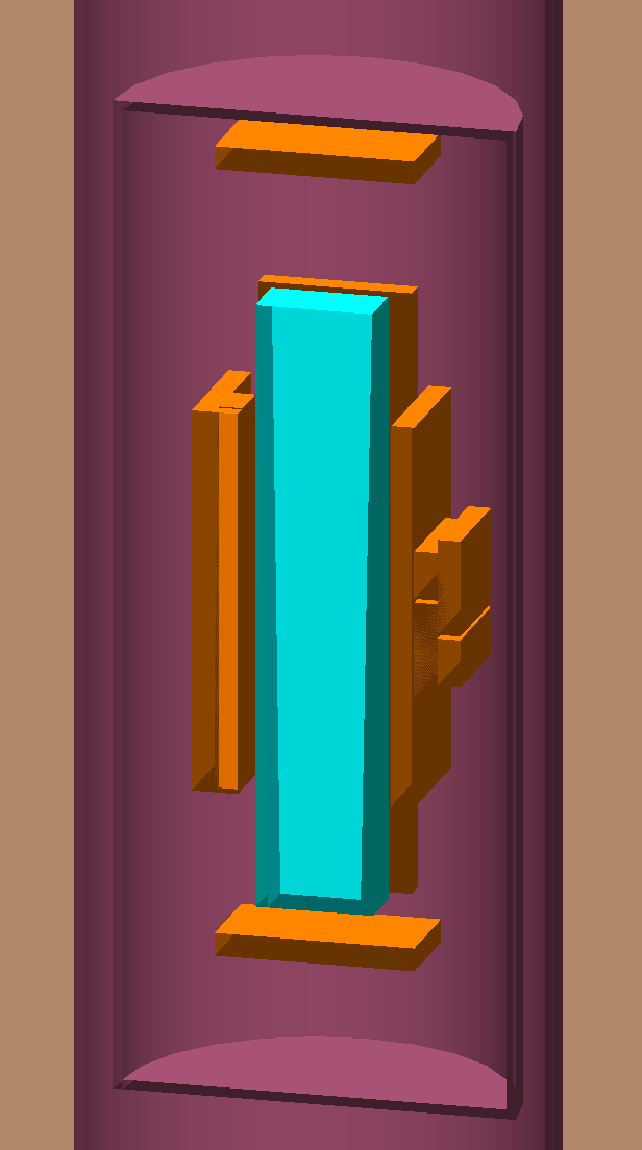
\includegraphics[width=2.99cm]{figs/gemc-3d.pdf}  
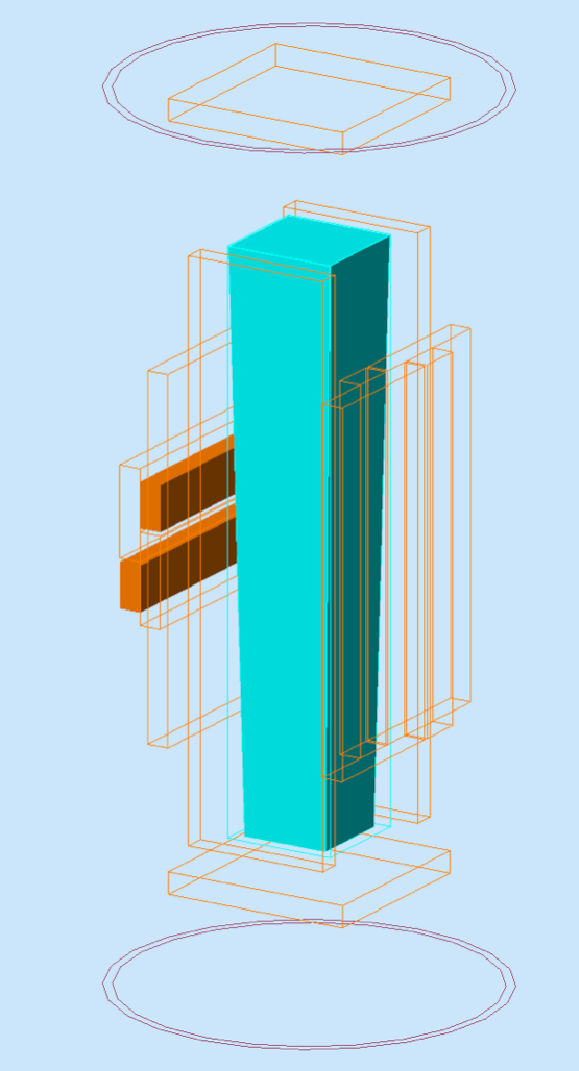
\includegraphics[width=2.9cm]{figs/gemc-3d1.pdf}  
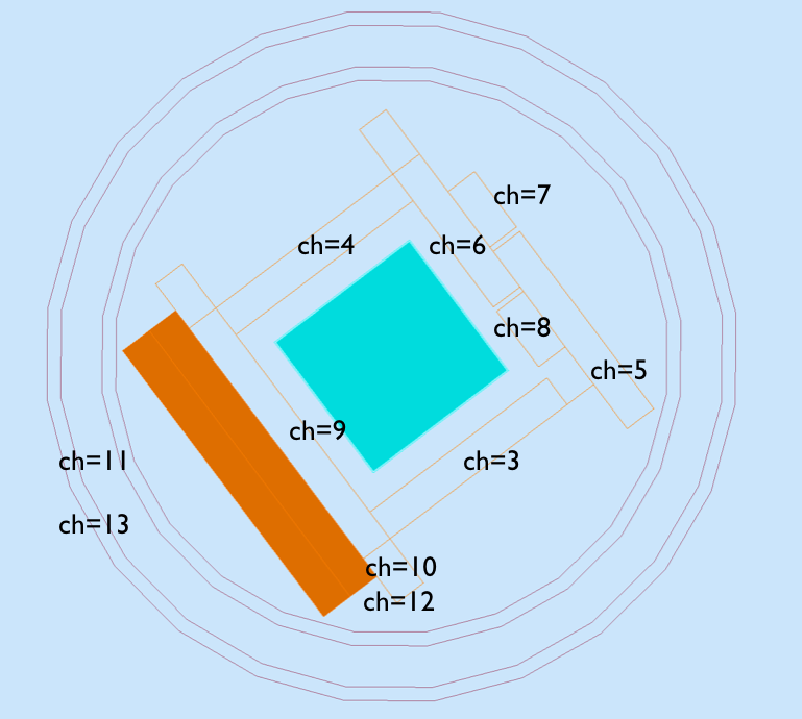
\includegraphics[width=6.0cm]{figs/gemc-3d2.pdf}  
\caption{The GEMC  implementation of the BDX-Hodo detector.}
\label{fig:det-gemc}
\end{figure}


The  detector geometry as well as the realistic response of the CsI(Tl) crystal and plastic scintillators have been implemented in GEMC (see  Appendix B.2 of PR-16-001~\cite{bdx-proposal} for details about the detectors response  parametrisation). 
Figure~\ref{fig:det-gemc} shows the BDX-Hodo implementation in GEMC. 
To estimate rates, we assumed a detection threshold of 10 phe in scintillators and 100 phe in the crystal corresponding to 400 keV and 2 MeV of deposited energy respectively\footnote{MIPs release $\sim50$ phe ($\sim$2 MeV) and 1670 phe ($\sim$32 MeV)  respectively.}. 


